 \appendix
 \section{Proofs of NP-hardness} \label{sec:np}
 \subsection{Enforcement of Isolation Policies} \label{sec:isolationNP}
 Given a undirected graph $T=\{S,L\}$ which represents the switch topology denoted in \cref{fig:swtopo} and undirected graph $P =\{R,I\}$ which represents the policy graph. Every vertex $r \in R$ is a reachability policy : $s >> d$ and each edge $i \in I$ which connects vertices $r1$ and $r2$ mean that the paths of $r1$ and $r2$ are isolated from each other. 
 \begin{figure}[H] 
 	\centering
 	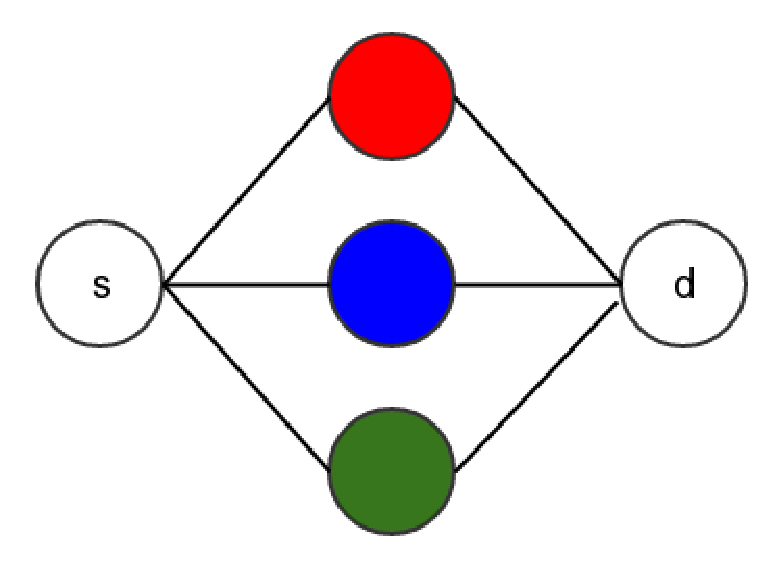
\includegraphics[width=0.7\columnwidth]{figures/color_topo.eps}
 	\caption{The switch topology $T$. All circles represent switches and all reachability policies are $s$ to $d$}
 	\label{fig:swtopo}
 \end{figure}
The solution to policy enforcement will be such that each reachability policy $r \in R$ from $s >> d$ will traverse through one of the colored switches $\{red$, $blue$, $green\}$. Color the vertices $R$ with the switch the path traverses through. If two vertices are connected by an edge in $I$, those flows would be isolated, and thus, will not have the same color. Thus, the problem reduces to finding a 3-graph coloring for the graph which is NP-complete. Thus, the enforcement of isolation policies is NP-complete. 
 
 In genral, k-coloring (for k > 2) is NP-complete and k-coloring problem reduces into a policy enforcement problem in a switch topology with k paths from source to destination, and thus, isolation policy enforcement is NP-complete. 
Similarly, The Hamiltonian Path problem can be reduced to an unordered waypoint policy, and thus, finding a path with unordered waypoints is NP-complete. The proof for this is omitted in this paper. 
 
% \subsection{Enforcement of Waypoint Policies}
% Given a undirected graph $G={V,E}$. Let us assume there exists an polynomial-time algorithm to compute the reachability paths satisfying the policies of the following types on the graph : \\
% \begin{itemize} 
% 	\item \textbf{P1} : $v_1 >> v_2 \Rightarrow$ There exists a path from $v_1$ to $v_2$ satisfying all input policies. A property of the path is that it does not have repeat a vertex (no forwarding loops).
% 	\item \textbf{P2} : $v_1 >> W >> v_2 \Rightarrow$ The path from $v_1$ to $v_2$  should pass through the vertices in the set $W$ in any order, without repeating a vertex.
% \end{itemize}
% \textbf{Reduction of Hamiltonian Cycle Problem} : Given a undirected graph $G={V,E}$, find $v \in V$ such that the degree of $v$ is the minimum in the graph (Will work for any vertex actually). If a Hamiltonian cycle is present in the graph, it will have the vertex $v$ in the cycle, and one of the edges from $v$.  \\
% Lets take a $n \in Neighbours(v)$. Let the input policies to our algorithm be : 
% \begin{itemize}
% 	\item \textbf{P4} : $v >> W >> n$ where $W = V - \{v,n\} $ 
% \end{itemize}
%P4 cimputes a simple path from $v$ to $n$ which passes through all the other vertices in the graph which is the Hamiltonian path problem. Since computing the Hamiltonian path is NP-hard, the problem of path computation for the waypoint policies as specified is NP-hard. 